\subsubsection{\Optimizing MSVC 2010}

\lstinputlisting[caption=\Optimizing MSVC 2010]{patterns/12_FPU/3_comparison/x86/MSVC_Ox/\LANG.asm}

\index{x86!\Instructions!FCOM}
\RU{\FCOM отличается от \FCOMP тем что просто сравнивает значения и оставляет стек в том же состоянии. 
В отличие от предыдущего примера, операнды здесь в другом порядке. 
Поэтому и результат сравнения в \CThreeBits будет другим чем раньше:}
\EN{\FCOM is distinguished from \FCOMP in that sense that it just comparing values and leaves FPU stack 
in the same state. 
Unlike previous example, operands here in reversed order. 
And that is why result of comparison in the \CThreeBits will be different:}

\begin{itemize}
\item
\RU{Если a>b в нашем случае, то биты \CThreeBits должны быть выставлены так:}
\EN{If a>b in our example, then \CThreeBits bits will be set as:} 0, 0, 0.
\item
\RU{Если b>a, то биты будут выставлены:}\EN{If b>a, then bits will be set as:} 0, 0, 1.
\item
\RU{Если a=b, то биты будут выставлены так:}\EN{If a=b, then bits will be set as:} 1, 0, 0.
\end{itemize}
% TODO: table?

\RU{Инструкция \TT{test ah, 65} как бы оставляет только два бита ~--- \Cthree и \Czero. 
Они оба будут нулями, если a>b: в таком случае переход \JNE не сработает. 
Далее имеется инструкция \TT{FSTP ST(1)} ~--- эта инструкция копирует 
значение \ST{0} в указанный операнд и выдергивает одно значение из стека. В данном случае, 
она копирует \ST{0} 
(где сейчас лежит \TT{\_a}) в \ST{1}. 
После этого на вершине стека два раза лежат \TT{\_a}. Затем одно значение выдергивается. 
После этого в \ST{0} остается \TT{\_a} и функция завершается.}
\EN{It can be said, \TT{test ah, 65} instruction just leaves two bits~---\Cthree and \Czero. 
Both will be zeroes if \TT{a>b}: in that case \JNE jump will not be triggered. 
Then \TT{FSTP ST(1)} is following~---this instruction copies value in the \ST{0} into operand and 
popping one value from FPU stack.
In other words, the instruction copies \ST{0} (where \TT{\_a} value is now) into the \ST{1}.
After that, two values of the {\_a} are at the top of stack now. 
After that, one value is popping.
After that, \ST{0} will contain {\_a} and function is finished.}

\RU{Условный переход \JNE сработает в двух других случаях: если b>a или a==b. 
\ST{0} скопируется в \ST{0}, что как бы холостая операция, 
затем одно значение из стека вылетит и на вершине стека останется то что 
до этого лежало в \ST{1} (то есть, \TT{\_b}). И функция завершится. 
Эта инструкция используется здесь видимо потому что в FPU нет инструкции которая просто выдергивает 
значение из стека и выбрасывает его.}
\EN{Conditional jump \JNE is triggered in two cases: of b>a or a==b. 
\ST{0} into \ST{0} will be copied, it is just like idle (\ac{NOP}) operation, then one value 
is popping from stack and top of stack (\ST{0}) will contain what was in the \ST{1} before 
(that is {\_b}). Then function finishes. 
The instruction used here probably since \ac{FPU} has no instruction to pop value from stack and 
discard it.}

\paragraph{\RU{Первый пример с \olly}\EN{First \olly example}: a=1.2 \AndENRU b=3.4}

\RU{Обе}\EN{Both} \FLD \RU{отработали}\EN{executed}: \figref{fig:FPU_comparison_Ox_case1_olly1}.
\RU{Сейчас будет исполняться }\FCOMP\EN{ being executed}: 
\olly \RU{показывает содержимое}\EN{shows contents of} \ST{0} \AndENRU \ST{1}, \RU{для удобства}
\EN{for convenience}.

\FCOM \RU{сработала}\EN{is done}: \figref{fig:FPU_comparison_Ox_case1_olly2}.
\Czero \RU{установлен, остальные флаги сброшены}\EN{is set, all other condition flags are cleared}.

\FNSTSW \RU{сработала}\EN{is done}, \TT{AX}=0x3100: \figref{fig:FPU_comparison_Ox_case1_olly3}.

\TEST \RU{сработала}\EN{executed}: \figref{fig:FPU_comparison_Ox_case1_olly4}.
ZF=0, \RU{переход сейчас произойдет}\EN{conditional jump will trigger now}.

\TT{FSTP ST} (\OrENRU \FSTP \ST{0}) \RU{сработала}\EN{executed}: $1.2$ 
\RU{было вытолкнуто из стека, и на вершине осталось $3.4$}\EN{was popped from the stack,
and $3.4$ was left on top of it}.
\figref{fig:FPU_comparison_Ox_case1_olly5}.
\RU{Видно, что инструкция}\EN{We see that the} \TT{FSTP ST} 
\RU{работает просто как выталкивание одного значения из FPU-стека}
\EN{instruction works just like popping one value from FPU-stack}.

\begin{figure}[H]
\centering
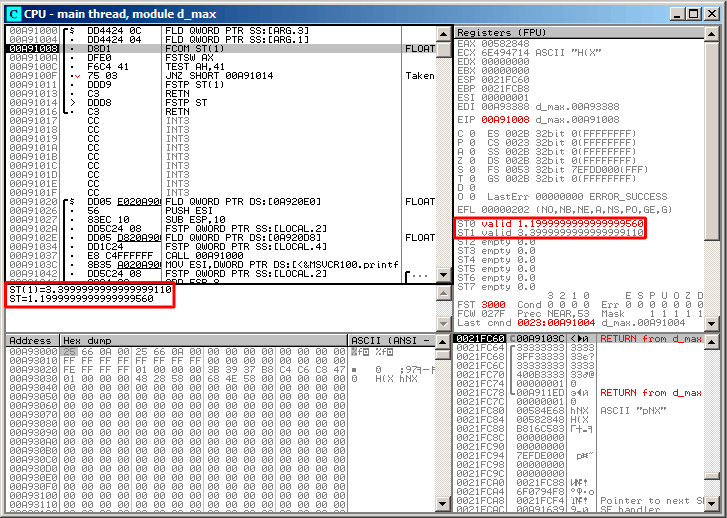
\includegraphics[scale=\FigScale]{patterns/12_FPU/3_comparison/x86/MSVC_Ox/olly1_1.png}
\caption{\olly: \RU{обе \FLD исполнились}\EN{both \FLD executed}}
\label{fig:FPU_comparison_Ox_case1_olly1}
\end{figure}

\begin{figure}[H]
\centering
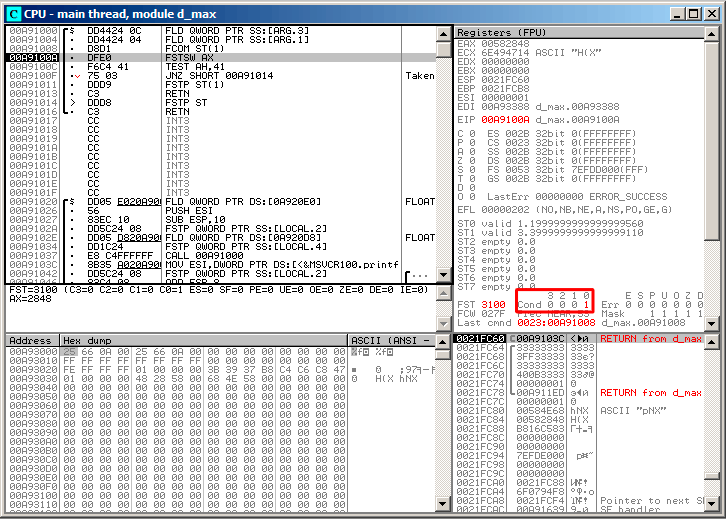
\includegraphics[scale=\FigScale]{patterns/12_FPU/3_comparison/x86/MSVC_Ox/olly1_2.png}
\caption{\olly: \FCOM \RU{исполнилась}\EN{executed}}
\label{fig:FPU_comparison_Ox_case1_olly2}
\end{figure}

\begin{figure}[H]
\centering
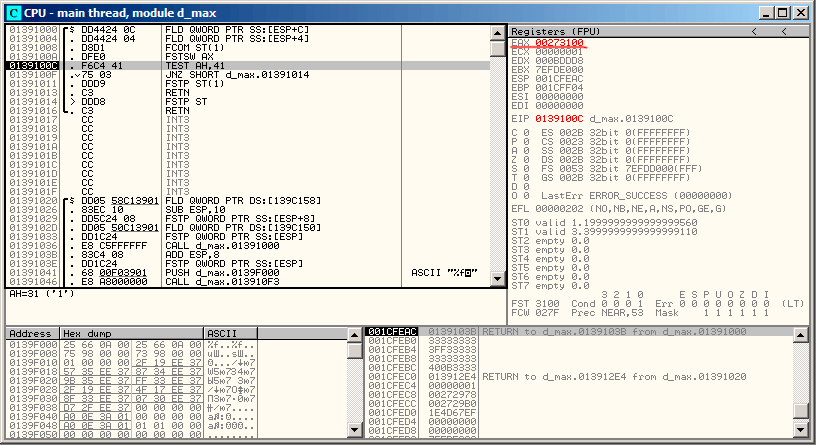
\includegraphics[scale=\FigScale]{patterns/12_FPU/3_comparison/x86/MSVC_Ox/olly1_3.png}
\caption{\olly: \FNSTSW \RU{исполнилась}\EN{executed}}
\label{fig:FPU_comparison_Ox_case1_olly3}
\end{figure}

\begin{figure}[H]
\centering
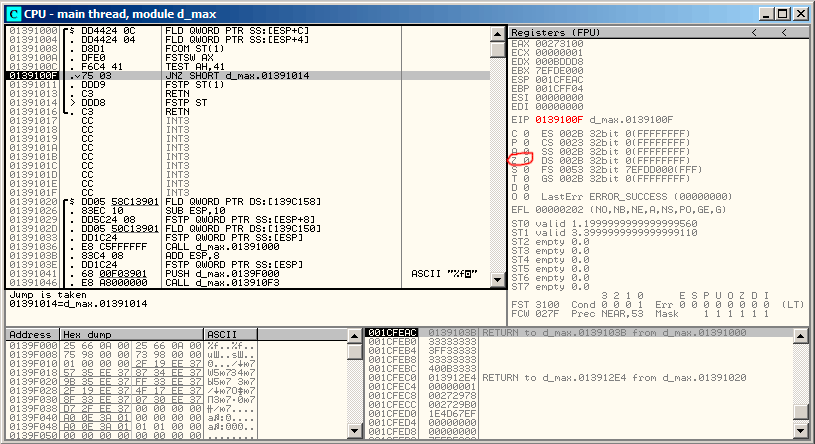
\includegraphics[scale=\FigScale]{patterns/12_FPU/3_comparison/x86/MSVC_Ox/olly1_4.png}
\caption{\olly: \TEST \RU{исполнилась}\EN{executed}}
\label{fig:FPU_comparison_Ox_case1_olly4}
\end{figure}

\begin{figure}[H]
\centering
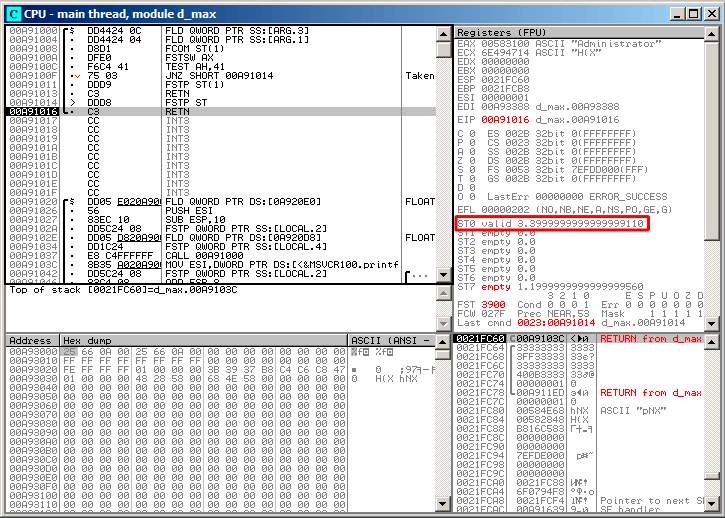
\includegraphics[scale=\FigScale]{patterns/12_FPU/3_comparison/x86/MSVC_Ox/olly1_5.png}
\caption{\olly: \FSTP \RU{исполнилась}\EN{executed}}
\label{fig:FPU_comparison_Ox_case1_olly5}
\end{figure}

\paragraph{\RU{Второй пример с \olly}\EN{Second \olly example}: a=5.6 \AndENRU b=-4}

\RU{Обе}\EN{Both} \FLD \RU{отработали}\EN{executed}: \figref{fig:FPU_comparison_Ox_case2_olly1}.
\RU{Сейчас будет исполняться }\FCOMP\EN{ being executed}.

\FCOM \RU{сработала}\EN{done}: \figref{fig:FPU_comparison_Ox_case2_olly2}.
\RU{Все condition-флаги сброшены}\EN{All condition-flags are cleared}.

\FNSTSW \RU{сработала}\EN{done}, \TT{AX}=0x3000: \figref{fig:FPU_comparison_Ox_case2_olly3}.

\TEST \RU{сработала}\EN{is done}: \figref{fig:FPU_comparison_Ox_case2_olly4}.
ZF=1, \RU{переход сейчас не произойдет}\EN{jump will not be triggered now}.

\FSTP \ST{1} \RU{сработала: на вершине FPU-стека осталось значение $5.6$}\EN{was executed: a value
of $5.6$ is now at the top of FPU-stack}.
\figref{fig:FPU_comparison_Ox_case2_olly5}.
\RU{Видно, что инструкция}\EN{We now see that} \FSTP \ST{1} 
\RU{работает так: оставляет значение на вершине стека, но обнуляет регистр \ST{1}}
\EN{instruction works as follows: it leaves what was at the top of stack, but clears \ST{1} register}.

\begin{figure}[H]
\centering
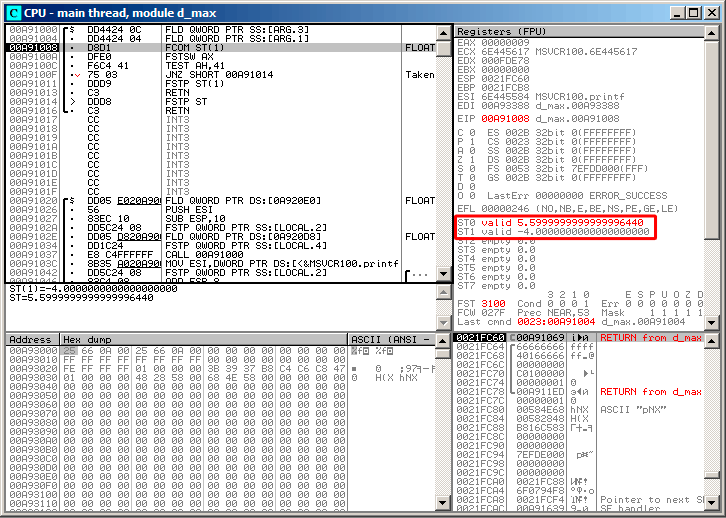
\includegraphics[scale=\FigScale]{patterns/12_FPU/3_comparison/x86/MSVC_Ox/olly2_1.png}
\caption{\olly: \RU{обе \FLD исполнились}\EN{both \FLD executed}}
\label{fig:FPU_comparison_Ox_case2_olly1}
\end{figure}

\begin{figure}[H]
\centering
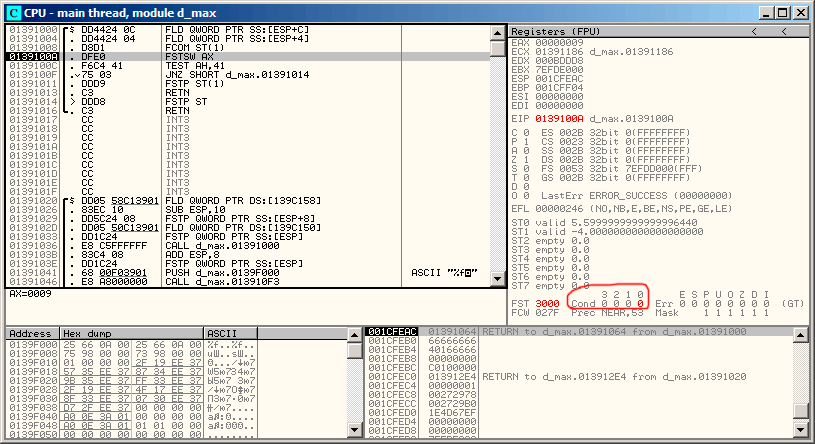
\includegraphics[scale=\FigScale]{patterns/12_FPU/3_comparison/x86/MSVC_Ox/olly2_2.png}
\caption{\olly: \FCOM \RU{исполнилась}\EN{executed}}
\label{fig:FPU_comparison_Ox_case2_olly2}
\end{figure}

\begin{figure}[H]
\centering
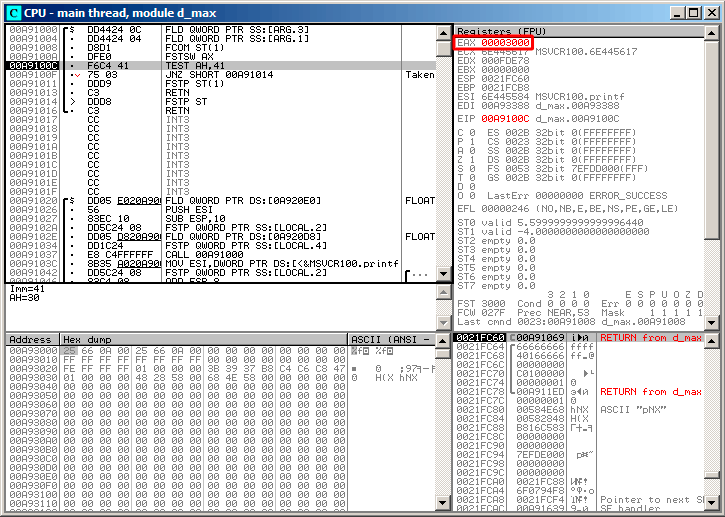
\includegraphics[scale=\FigScale]{patterns/12_FPU/3_comparison/x86/MSVC_Ox/olly2_3.png}
\caption{\olly: \FNSTSW \RU{исполнилась}\EN{executed}}
\label{fig:FPU_comparison_Ox_case2_olly3}
\end{figure}

\begin{figure}[H]
\centering
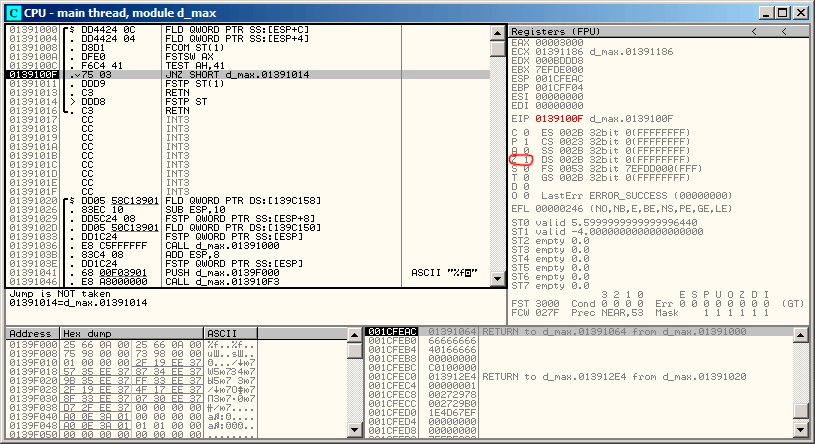
\includegraphics[scale=\FigScale]{patterns/12_FPU/3_comparison/x86/MSVC_Ox/olly2_4.png}
\caption{\olly: \TEST \RU{исполнилась}\EN{executed}}
\label{fig:FPU_comparison_Ox_case2_olly4}
\end{figure}

\begin{figure}[H]
\centering
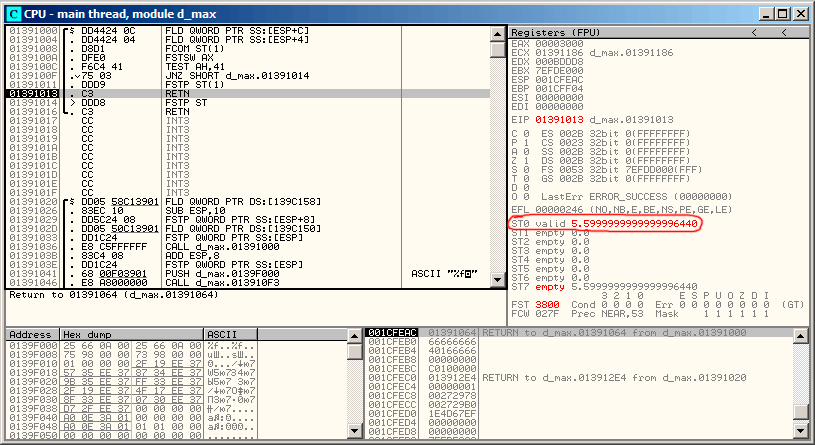
\includegraphics[scale=\FigScale]{patterns/12_FPU/3_comparison/x86/MSVC_Ox/olly2_5.png}
\caption{\olly: \FSTP \RU{исполнилась}\EN{executed}}
\label{fig:FPU_comparison_Ox_case2_olly5}
\end{figure}
